\documentclass[letterpaper,12pt,oneside]{book}
%\usepackage[a4paper,includeall,bindingoffset=0cm,margin=2cm,marginparsep=0cm,marginparwidth=0cm]{geometry}
\usepackage[top=1in, left=0.9in, right=1.25in, bottom=1in]{geometry}
\usepackage{bachelorstitlepageUNAM}
\usepackage[utf8]{inputenc}
%%%%%%%%%%%%%%%%%%%%%%%%%%%%%
% Comparto una plantilla para la PORTADA que us\'e en mi t\'esis
% basada en el dise\~no gen\'erico que se usa en la Facultad de Ciencias
% Para usarlo \'unicamente aseg\'urate de tener la l\'inea
% \usepackage{bachelorstitlepageUNAM} y el archivo bachelorstitlepageUNAM.sty en el mismo directorio de trabajo.
% y los campos (sin signo %) :
%\author{Nombre del Alumno}
%\title{T\'itulo de la tesis}
%\faculty{Facultad}
%\degree{Grado que obtienes}
%\supervisor{ Tutor}
%\cityandyear{Ciudad y anio}
%\logouni{nombredelescudodelaunamsinespacios}
%\logofac{NombreDeLaImagenDelEscudodeTuFacultadSinEspacios}
% Para sugerencias y comentarios: DM en twitter.com/sglvgdor
% Subir\'e mas adelante la plantilla para maestr\'ia
%%%%%%%%%%%%%%%%%%%%%%%%%%%%%

%\author{Irving Yosafat Angel Camacho}
%\title{Métodos Numéricos de la Hidrodinámica Relativista aplicados a problemas de acreción y eyección en %jets astrofísicos}
%\faculty{Escuela Nacional de Estudios Superiores\\
%            Unidad Morelia}
%\degree{Licenciado en Geociencias}
%\supervisor{Dr. Sergio Mendoza Ramos \\ 
%Dr. Sinhué A. R. Haro Corzo}
%\cityandyear{Morelia, Michoacán, 2019}
%\logouni{Escudo-UNAM}
%\logofac{logo-enes}
%
%-------------------------------

%###################################
% Artículo 12.- El protocolo de tesis, con el visto bueno de un asesor, deberá ser entregado por 
% el alumno a la Coordinación de Carrera correspondiente para su registro, así como para su 
% presentación ante el Comité de Aprobación de Protocolo de Tesis correspondiente. El alumno 
% deberá tener un mínimo del 90% de créditos de su carrera para registrar su protocolo. La 
% Coordinación de Carrera será la responsable de realizar las gestiones académico-administrativas de 
% esta opción de titulación.
% Para someter el protocolo de tesis al Comité de Aprobación de Protocolo de Tesis respectivo, se 
% deberá entregar un documento que no exceda de cinco cuartillas, además de la portada, 
% considerando el contenido siguiente:
%    a) Portada, la cual deberá incluir: título del trabajo de tesis, nombre del alumno y nombre del asesor;
%    b) Objetivo(s) del trabajo;
%    c) Índice tentativo del trabajo de tesis;
%    d) Introducción, antecedentes y justificación del trabajo;
%    e) Metodología a emplear, y
%    f) Bibliografía básica (mínimo 10 referencias)
%###################################
\usepackage{float}
\newcommand{\figura}[4]
{
  \begin{figure}[H]
    \centering
    \includegraphics[scale=#1]{#2}
    \caption{#3}
    \label{#4}
  \end{figure}
}
\newcommand{\refig}[1]{\figurename~\ref{#1}}
\newcommand{\refeq}[1]{\textbf{ec.}~\ref{#1}}
\newcommand{\reteo}[1]{$\mathfrak{Teorema}$~\ref{#1}}
\newcommand{\bb}[1]{\{#1\}}

%%Definiciones matemáticas
%\newtheorem{defi}{{\it Definici\’on}}[chapter]
\newtheorem{defi}{\textit{\textmd{$\mathfrak{Definición}$} }}
\newtheorem{teo}{\textit{\textmd{$\mathscr{TEOREMA}$} }}


%-----------------------__--------

\usepackage[T1]{fontenc}
\usepackage[utf8]{inputenc}
\usepackage[spanish,es-nodecimaldot,es-tabla]{babel}
\usepackage{graphicx}
\usepackage{tikz} 
\usepackage{tocloft}
\graphicspath{{./figs/}}
\usepackage{setspace}
\usepackage[nottoc]{tocbibind}
%\usepackage[round]{natbib}

\renewcommand\cftsecpresnum{\S}
\renewcommand\cftsubsecpresnum{\S}   


\begin{document}
%------------------------------

    \begin{titlepage}
        \thispagestyle{empty}
        \begin{minipage}[c][0.17\textheight][c]{0.25\textwidth}
            \begin{center}
                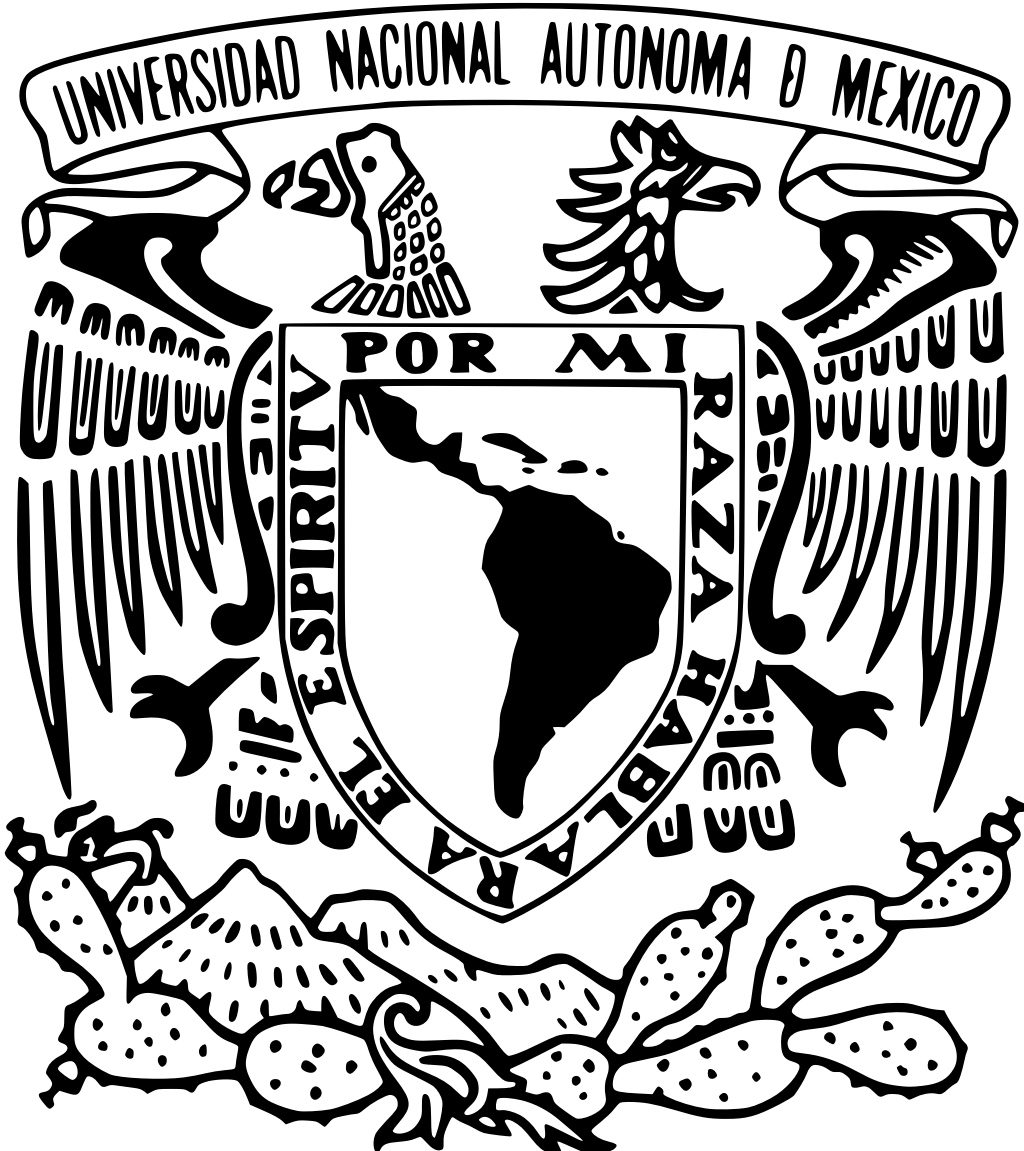
\includegraphics[width=3.5cm, height=4cm]{/home/aceron/Documentos/GitHub/Tesis/docTesis/Escudo-UNAM.png}
            \end{center}
        \end{minipage}
        \begin{minipage}[c][0.195\textheight][t]{0.75\textwidth}
            \begin{center}
                \vspace{0.3cm}
                \textsc{\large Universidad Nacional Aut\'onoma de M\'exico}\\[0.5cm]
                \vspace{0.3cm}
                \hrule height2.5pt
                \vspace{.2cm}
                \hrule height1pt
                \vspace{.8cm}
                \textsc{CENTRO DE FÍSICA APLICADA Y TECNOLOGÍA AVANZADA}\\[0.5cm] %
            \end{center}
        \end{minipage}

        \begin{minipage}[c][0.81\textheight][t]{0.25\textwidth}
            \vspace*{5mm}
            \begin{center}
                \hskip2.0mm
                \vrule width1pt height13cm 
                \vspace{5mm}
                \hskip2pt
                \vrule width2.5pt height13cm
                \hskip2mm
                \vrule width1pt height13cm \\
                \vspace{5mm}
                
\includegraphics[height=4.0cm]{/home/aceron/Documentos/GitHub/Tesis/docTesis/Esculo-CFATA.png}
            \end{center}
        \end{minipage}
        \begin{minipage}[c][0.81\textheight][t]{0.75\textwidth}
            \begin{center}
                \vspace{1cm}

                {\large\scshape (Título tentativo) Estudio de la viabilidad de sistemas de recolección de agua de lluvia en el Estado de Querétaro usando datos del radar meteorológico ubicado en el Cerro de la Ronchera}\\[.2in]

                \vspace{2cm}            

                %\textsc{\LARGE T\hspace{1.5cm}E\hspace{1.5cm}S\hspace{1.5cm}I\hspace{1.5cm}S}\\[0.5cm]
                %\textsc{\large que para obtener el t\'itulo de:}\\[0.5cm]
                %\textsc{\large Licenciado en Tecnología}\\[0.5cm]
                \textsc{\large Protocolo de Tesis}\\[0.5cm]
                \textsc{\large presenta:}\\[0.5cm]
                \textsc{\large {Ariel Cerón González}}\\[2cm]          

                \vspace{0.5cm}

                {\large\scshape Tutores:\\[0.3cm] {Dr. Adolfo Magaldi Hermosillo}}\\[.2in]

                \vspace{0.5cm}

                \large{Querétaro, Querétaro}{ }{2021}
            \end{center}
        \end{minipage}
    \end{titlepage}



%---------------------------------
\frontmatter
%\maketitle
% \chapter*{}
% \begin{flushright}%
%   \emph{Dedicatoria ...}
%   \thispagestyle{empty}
% \end{flushright}

% \chapter{Agradecimientos}
% \spacing{1.5}%\doublespacing

%\chapter{Notación}

\chapter{Introducción}
    La administración de los recursos hídircos es un tema de gran interés para diferentes sectores, por los beneficios económicos y de salud que genera.

    Actualmente, México enfrenta varias problemáticas entorno al recurso hídirco entre las que se encuentran: falta de acceso al recurso, la mala calidad del recurso, la deficiencia de lluvias (originados por la tala inmoderada y la destrucción de ecosistémas), exceso de concesiones del recurso \cite{jornada:agua}, y la falta de mantenimiento a la infraestructura existente.

    Aunque en los últimos años se ha reconocido la importancia de cuidar y administrar el recurso \cite{de2019objetivo} \cite{mex:procaptar} son pocas las propuestas tecnologías implementadas para minimizar alguno de los problemas mencionados.
    Una de las soluciones más reproducida, es la captación del agua de lluvia en zonas urbanas\cite{comision2016lineamientos} \cite{hugues2019captacion} \cite{nickisch2018sistemas} \cite{van2013captacion} las cuales se pueden resumir en la implementación y combinación de tres sistemas, a saber, un sistema recolector, un sistema de transporte y un sistema de almacenamiento; sin embargo pocas soluciones consideran aspectos meteorológicos para su aplicación.

    El aprovechamiento de instrumentos meteorológicos, como el radar meteorológico, podrían dotar de información que permita validar la eficiencia de los sistemas recolectores, sin la necesidad de realizar una instalación, ahorrando costos en la implementación del sistema. Por otro lado, los campos de precipitación obtenidos mediante el radar meteorológico pueden ser considerados para la implementación de mejores políticas de gestión pública del recurso y para la planeación urbana.
\newpage
    \section{Hipótesis}
        Los registros históricos del radar meteorológico pueden proveer información sobre la distribución de precipitación pluvial temporal y espacial. El correcto uso de los datos permitirá observar la evolución de la precipitación y la capacidad que tiene el estado para su aprovechamiento.

    \section{Objetivos}
        Conocer el comportamiento historio de la precipitación pluvial registrada con datos del radar meteorológico ubicado en el Cerro de la Ronchera para validar sistemas de recolección y almacenamiento de agua de lluvia.
        \subsection{Particulares}
            \begin{itemize}
                \item Generar mapas hídricos del estado de Querétaro para diferentes años y temporadas del año.
                \item Conocer y pronosticar la demanda hídrica del estado de Querétaro.
            \end{itemize}

    \section{Justificación}
        El estado de Querétaro ha presentado un crecimiento poblacional acelerado en los últimos años, lo que trae consigo mayor demanda de recursos básicos, entre ellos el acceso al agua, la cual se ha visto comprometido en los últimos años.
        La alta demanda y la deficiencia del recurso generan la necesidad de contar con alternativas que permitan a la población acceso al recurso. Uno de los métodos más populares es el de la cosecha de lluvia, sin embargo la orografía y el clima del estado plantea una problemática al momento de implementar esta solución. Si se pueden conocer las necesidades hídricas en cada municipio del estado, así como la cantidad de precipitación se facilitaría la implementación de tecnologías y políticas que permitan generar una mayor resiliencia a la escases de agua. Esto puede ser cálculado usando los datos del radar meteorológico de la Comisión Estatal de Aguas de Querétaro (CEA) ubicado en el Cerro de la Ronchera.
\newpage
\chapter*{Antecedentes} 
    El estado de Querétaro ha desarrollado problemas sobre la disponibilidad de recursos hídricos necesarios para satisfacer a la población, la industria y la agricultura. 
    
    La disponibilidad del agua es un elemento importante para el bienestar económico y social de ciudad, y no solo el abasto sino que ésta debe ser de calidad aceptable, en cantidad adecuada y continua y a un precio razonable.
    
    Una forma para garantizar más años de acceso al agua es el uso sostenible de los recursos hídircos, para ello es necesario aprovechar todas las fuentes existentes, optimizando su suministro, concientizando su consumo y promoviendo su conservación. Sin embargo, el hecho de que el abastecimiento del agua potable de la zona metropolitana de la ciudad de Querétaro (ZMCQ) provenga principalmente de un acuífero subterráneo sobre-explotado -Acuífero del Valle de Querétaro- refleja una precariedad en la definición de sostenible y representa un riesgo considerable para el gobierno y la sociedad, haciendo inevitable desarrollar estrategias y acciones específicas para garantizar el abasto de agua a largo plazo. Para lograr el abasto de agua sostenible es necesario generar la sustentabilidad\footnote{El desarrollo equitativo que cumple las necesidades del presente sin comprometer la habilidad de las generaciones futuras para cumplir sus propias necesidades} pasando por la conservación de sus fuentes como la lluvia, acuíferos, lagos, rios y bosques hasta llegar a la planeación completa del consumo y su distribución, fomentando el ahorro del recurso y aprovechar al máximo, sin sobreexplotar, las fuentes locales.

    Un método popular de aprovechamiento (reflejado en las diferentes tésis y manuales \cite{comision2016lineamientos} \cite{hugues2019captacion} \cite{nickisch2018sistemas} \cite{van2013captacion},\cite{queralt2011agua} \cite{unatsabar2004guia}) es el de la captación de agua de lluvia, el cual consiste en la implementación de tres móodulos especializados: uno de captación, uno de transporte y un último de almacenamiento. Sistemás más complejos incluyen  eliminación de bacterias, separación de partículas pesadas o circulación inteligente del recurso.

\chapter*{Metodología}
    La Organización Meteorológica Mundial \cite{omm2014guia} establece diferentes métodos para la medición de la precipitación. En este trabajo, usaremos la información generada por un radar meteorológico Doppler la cual, consiste en registrar el valor de reflectividad generada por la reflección de energía de un blanco (hidrometeóros) al interceptar un pulso electromagnético emitido por el radar,  y aplicaremos la relación $Z-R$ (\refeq{eq:eq1}) que transforma los valores de reflectividad en precipitación acumulada.
    \begin{equation}
        Z= aR^b
        \label{eq:eq1}
    \end{equation}
    Los registros de reflectividad en un radar varia en función del tiempo que tarda en generar un mapeo\footnote{Un radar emite un pulso en un cierto ángulo de inclinación (azimuth) y en un cierto ángulo de rotación. Cuando se termina una ratoción el ángulo de inclinación se modifica y, cuando se llega a la inclinación máxima se reinicia el proceso de mapeo.}, normalmente la frecuencia de adquisición de datos para un mismo punto varia entre los 10 y 20 minutos. Sabiendo esto, se realizará una acumulación diaria ($S$) siguiendo la \refeq{eq:eq2}, donde $Z_i$ es un arreglo de valores de precipitación en un tiempo dado y $n$ es la cantidad registros existentes para un día. Si se repite está operación se puede construir otras temporalidades como: semanal, mensual y anual.
    %Ya que el número de datos registrados por un radar varía en función del tiempo que tarda en generar un mapeo\footnote{Un radar emite un pulso en un cierto ángulo de inclinación (azimuth) y en un cierto ángulo de rotación. Cuando se termina una ratoción el ángulo de inclinación se modifica y, cuando se llega a la inclinación máxima se reinicia el proceso de mapeo.}, normalmente la frecuencia de adquisición de datos para un mismo punto varia entre los 10 y 20 minutos, haciendo necesario un procesamiento de transformación y acumulación para conocer la precipitación en espacios temporales mayores. Para ello se usará una ecuaión de la forma \ref{eq:eq2}, con $n$ la cantidad de datos y $Z_i$ el valor de precipitación acumulada para el dato $i$
    \begin{equation}
        S= \sum^n Z_i
        \label{eq:eq2}
    \end{equation}
    
    Aunado a esto se trabajarán con los datos de consumo que la Comisión Estatal de Aguas de Querétaro (CEA) tiene  registrado para diferentes sectores (urbano, agricola, industria, privado); con estos, se espera conocer con estos datos la necesidad hídrica de la población y con esto generar descriptores de consumo, para cada uno de los sectores que define la CEA, que serán de ayuda al momento de validar los sistemas.

    Una vez generada la información de precipitación se construirán mapas hidrícos en diferentes periodos estacionales que describan la capacidad de precipitación en cada zona del estado. Con ello se pretende conocer si la precipitación de cada zona cubre a los descriptores generados con anterioridad.
    %\figura{0.5}{/home/aceron/Documentos/GitHub/Tesis/docTesis/metodo.png}{Diagrama de proceso}{fig:fig1}
\newpage
\tableofcontents
%\listoffigures

\mainmatter

\chapter{Antecedentes.} 
\chapter{El agua y su consumo.}
    \section{El agua en Querétaro.}
        \subsection{Hidrología.}
        \subsection{Clima.}
        \subsection{Consumidores.}
        \subsection{Crisis.}
\chapter{Precipitación Pluvial.} 
    \section{Proceso de precipitación.}
        \subsection{Nubes.}
        \subsection{Precipitación.}
    \section{Métodos de medición.}
        \subsection{Pluviómetros.}
        \subsection{Medidores de precipitación registradores.}
\chapter{Radar Meteorológico.}
    \section{Funcionamiento.}
    \section{Aplicación en la meteorología.}
\chapter{Metodología.}
    \section{Adquisición de datos.}
    \section{Procesamiento de la información.}
    \section{Estadística descriptiva.}
    \section{Validación de los resultados}
        \subsection{Creación de una medida de consumo.}
        \subsection{Creación de áreas de recolección.}
\chapter{Resultados.}
    \section{Datos meteorológicos.}
        \subsection{Mapas estacionales.}
    \section{Datos de consumo.}
        \subsection{Evolución temporal.}
    \section{Comparación entre el consumo y lo recolectado.}
\chapter{Conclusiones.}

%\chapter{Conclusiones}  
\nocite{*}
\bibliographystyle{apalike}
\bibliography{bibfile.bib}

\backmatter%@sglvgdor


\end{document}